\documentclass[12pt,letterpaper,twoside]{amsart}
\usepackage[latin1]{inputenc}
\usepackage{amsmath}
\usepackage{amsfonts}
\usepackage{graphicx}
\usepackage{amssymb}
\usepackage{multicol}
\usepackage{ulem}
\newcounter{example}
\newcounter{exercise}
\newcounter{problem}
\newtheorem{theorem}{Theorem}
\renewcommand{\proof}{{\bf Proof:}}
\newcommand{\example}{\bigskip \noindent {\large {\sc Example \arabic{example}:}} \addtocounter{example}{1}}
\newcommand{\exercise}{\bigskip \noindent {\large {\sc Exercise \arabic{exercise}:}} \addtocounter{exercise}{1}}
\newcommand{\problem}{\bigskip \noindent {\large {\sc Problem \arabic{problem}:}} \addtocounter{problem}{1}}
\newcommand{\tech}{\marginpar{\vskip 10mm \begin{center}\includegraphics[width=0.25in]{calculatorimagesmall.eps} \end{center}}}
\newcommand{\solution}{\medskip \noindent {\bf Solution: }}
\newcommand{\R}{\mathbb{R}}





\begin{document}

\sffamily

%%%%  switch the commenting on this line and the next \chapter{Introduction}
\begin{center} {\LARGE Existence and Uniqueness} \end{center}

\setcounter{example}{1}
\setcounter{exercise}{1}

Previously, we investigated the behaviour of solutions to various ODE.  The whole time, we assumed that there {\it were} solutions to the given equations.  Later, we will find approximate values for solutions of IVP using numerical methods which also assume that a solution exists.  But that assumption really requires proof if we are going to trust any of the conclusions we draw from the geometric approaches we took or the numerical methods we will employ later.  

The next theorem is the main result of this chapter.

\begin{theorem} Suppose that $f(y)$ and $f'(y)$ are defined and continuous on an open interval $(a,b)$ which contains $y_0$.  Then three is an open interval $I$ containing $x_0$ such that the initial value problem 
\[ \frac{dy}{dx}=f(y), \ \ \ y(x_0)=y_0\]
has a unique solution $y(x)$ defined on $I$.
\end{theorem}

We will prove this result in several stages, starting with the uniqueness part.  When we say that a solution to an IVP is unique on an interval $I$, we mean that if $y$ and $z$ are both functions that solve the IVP on $I$, then $y(t)=z(t)$ for all $t \in I$.  As the reader will find in the problems at the end of this chapter, uniqueness isn't always guaranteed.  But it is guaranteed (at least {\it near} $x_0$) when $f$ and $f'$ are both continuous.

The central idea in the uniqueness proof is a procedure called Picard iteration.  (This technique can also be used to prove existence, and this approach will be outlined in the problem set.)  Suppose that $y$ is a function defined on an interval $I$.  A {\bf Picard iterate} of $y$ is another function, $\tilde{y}$, defined according to the following formula:
\[ \tilde{y}(x) = y_0 + \int_{x_0}^x f(y(s)) \ ds\]

\exercise Suppose that $x_0=0$, $y_0=2$, $f(y)=y^2$ and $y(x)=x$.  Prove that $\tilde{y}(x)=2+\frac{s^3}{3}$.

\exercise Let $x_0=0$, $y_0=0$ and $f(y)=e^y$.  Find the Picard iterate of the function $y(x)=2x$.

\exercise Prove that $y(x)$ solves the initial value problem 
\[ \frac{dy}{dx}=f(y), \ \ \ y(0)=y_0\]
if and only if $\tilde{y}=y$.  {\it (Hint: Recall the Fundamental Theorem of Calculus.)}

The last exercise reveals the relationship between Picard iteration and initial value problems.  It allows us to recast the differential equation as an {\bf integral equation}: finding a solution $y(x)$ of the equation
\[ y(x)=y_0+\int_{x_0}^x f(y(s)) \ ds \]
is equivalent to finding a solution of the IVP $\frac{dy}{dx}=f(y), \ y(x_0)=y_0$.  The process below will illustrate how we go about verifying that the integral equation has a solution.

We need to define one more item of notation before we can proceed.  For a bounded function $f$ defined on an interval $I$, define
\[ \parallel f \parallel_I = \min \left\{ a; |f(x)|\leq a \mbox{ for all } x \in I \right\}.\]
This quantity is called the {\bf uniform norm} of $f$ on $I$, or just the {\bf norm} of $f$ for short.  Notice that if $|f|$ attains a maximum value on $I$, then $\parallel f \parallel_I = \max_{x \in I} |f(x)|$.

\exercise Let $f(x)=x^2-x$ on the interval $I=[0,1]$.  Prove that $\parallel f \parallel_I = \frac{1}{4}$.

\exercise Prove that if $\parallel f-g \parallel_I=0$, then $f(x)=g(x)$ for all $x \in I$.

The last exercise shows us how we can use the norm to identify when two functions are equal on a domain $I$: they are equal if the norm of their difference is zero.

\begin{theorem} Suppose that $|f'(y)| \leq K$, where $K \geq 0$ is some constant.  Then if the endpoints of the interval $I$ are $a$ and $b$, 
\[ \parallel \tilde{y} -\tilde{x} \parallel_I \leq K |b-a| \parallel y-z \parallel_I.\]
\label{contraction}
\end{theorem}

Notice that this theorem does not require that the interval $I$ be either open or closed.  $I$ may contain either endpoint $a$ or $b$, or both, or neither.

\proof 
For any $x \in I$ with $x \geq x_0$, we have
\begin{align*}
|\tilde{y}(x)-\tilde{z}(y)|
& = \left| y_0 + \int_{x_0}^x f(y(s)) \ ds - y_0 - \int_{x_0}^x f(z(s)) \ ds \right| \\
& = \left| \int_{x_0}^x (f(y(s)) - f(z(s))) \ ds \right| \\
& \leq \int_{x_0}^x |f(y(s))-f(z(s))| \ ds \\
& \leq \int_{x_0}^x K |y(s)-z(s)| \ ds \\
& \leq \int_{x_0}^x K \parallel y - z \parallel_I \ ds \\
& = K |x-x_0| \parallel y-z \parallel_I \\
& \leq K|b-a|\parallel y-z \parallel_I
\end{align*}
A small change to the calculation above shows that the same is true for $x \leq x_0$.  Since this inequality is true for all $x \in I$, it follows that 
\[\parallel \tilde{y}-\tilde{z} \parallel_I \leq K|b-a| \parallel y-z \parallel_I.\]
\qed

\exercise Modify the calculation in the proof above to deal with the case $x \leq x_0$.

\begin{theorem} Suppose that $f$ and $f'$ are defined and continuous on an open interval $(a,b)$ containing $y_0$.  Also suppose that  $|f'|<K$ on $(a,b)$, and $|b-a| < \frac{1}{K}$.  Then if $y_1$ and $y_2$ are both bounded functions that solve the IVP
\[ \frac{dy}{dx}= f(y), \ \ \ y(x_0)=y_0 \]
on the interval $I$, it must be true that $y_1(x)=y_2(x)$ for all $x \in I$.
\end{theorem}

\proof 
Let $L=K|b-a|$.  Then under the assumptions made here, we see that $L<1$.  Therefore we know that $\parallel \tilde{y_1} - \tilde{y_2} \parallel_I \leq L \parallel y_2 - y_1 \parallel_I.$  On the other hand, Ibecause $y_1$ and $y_2$ satisfy the IVP, it must be true that $\tilde{y_1}=y_1$ and $\tilde{y_2}=y_2$.  Putting these two facts together yields the inequality
\[ \parallel y_2-y_1 \parallel_I \leq L \parallel y_2-y_1 \parallel_I,\]
which can only be true if $\parallel y_2-y_1 \parallel_I = 0$ because we know $L < 1$.  (If this norm is not zero, divide both sides of the inequality by it to obtain $1 \leq L$, which would be a contradiction.)

Consequently, $y_2=y_1$ on $I$.
\qed

\begin{theorem} 
Suppose $f$ and $f'$ are defined on an interval $J$ containing $y_0$, and both functions are continuous on $J$.  Then there is an interval $I$ containing $x_0$ such that, if $y_2$ and $y_1$ are both solutions of 
\[ \frac{dy}{dx}=f(y), \ \ \ y(x_0)=y_0\]
on $I$, then $y_1=y_2$.
\end{theorem}
Another way to phrase the result of this theorem is that solutions of the IVP are unique in a neighborhood of $x_0$.

\proof
Because $f'$ is continuous at $y_0$, there is an open subinterval $\hat{J}$ of $J$ containing $y_0$ on which $f'$ is bounded.  Let 
\[K=\max_{z \in \hat{J}} |f'(z)|.\]
Let $a$ and $b$ denote the endpoints of $\hat{J}$, and define
\[ D=\min \{ |b-y_0|,|a-y_0| \},\]
so that $D$ is the minimum distance of $y_0$ from the endpoints of $\hat{J}$.  Define
\[ I = \left( x_0-\frac{D}{K}, x_0+\frac{D}{K} \right) .\]
Suppose that $y_1$ and $y_2$ are both solutions of the IVP on $I$.  For each $x \in I$,
\[ y_1(x)-y_0 = y_1(x)-y_1(x_0)=y_1'(x^*)(x-x_0)\]
for some $x^*$ between $x_0$ and $x$.  (This is a consequence of the mean value theorem.)  Thus $x^*$ is also contained in $I$, and therefore $|y'(x^*)|<K$.  Furthermore, $|x-x_0| \leq \frac{D}{K}$.  Consequently,
\[ |y_1(x)-y_0| = |y_1'(x^*)||x-x_0| < K \frac{D}{K}=D.\]
Since $|y_1(x)-y_0| < D$, it follows that $y_1(x) \in \hat{J}$ for all $x \in I$.  The same reasoning applies to $y_2$.  Now we can apply apply the previous theorem on the interval $I$ with the inequality $|f'|\leq K$ to obtain that $y_1=y_2$ on $I$.
\qed


With this last theorem, we have succeeded in proving the uniqueness part of Theorem 1.  It remains for us to prove that solutions do in fact exist.  It is possible to do this with Picard iteration -- in fact, for non-autonomous equations, that is exactly what we would need to do.  The idea is to define a sequence of functions $\{ y_i \}$, where each $y_i$ is the Picard iterate of $y_{i-1}$.  Then one proves that the sequence of functions $y_i$ converges to a function $y$ as $i \rightarrow \infty$, and then that this function $y$ is a solution.  This process is outlined in the problem set.

If we restrict our attention to autonomous equations here, we can use an alternative approach to proving existence which is somewhat easier.  The motivation for this proof is as follows.  If we were to try to solve the problem $\frac{dy}{dx}=f(y)$ using separation of variables, we'd end up with $\int \frac{1}{f(y)}\ dy = \int \ dx$, which is equivalent to the equation
\[ \int_{y_0}^y \frac{1}{f(s)} \ ds = x+C,\]
because, according to the Fundamental Theorem of Calculus, the left side is an anti-derivative of $\frac{1}{f(y)}$. 
Inserting the initial condition $x=x_0$ and $y=y_0$ yields $C=-x_0$, so we would have
\[ \int_{y_0}^y \frac{1}{f(s)} \ ds = x-x_0.\]
Finally, we would need to try to solve for $y$ in terms of $x$.  The following proof essentially verifies that the function $y(x)$ obtained in this way is indeed a solution of the IVP.


\begin{theorem} If $f$ is continuous on an open interval containing $y_0$, then there is a solution of the IVP
\[ \frac{dy}{dx}=f(y), \ \ \ y(x_0)=y_0\]
defined on an open interval containing $x_0$.
\end{theorem}

If $f(y_0)=0$, then the constant function $y(x)=y_0$ defined on $\mathbb{R}$ is a solution.  Now assume $f(y_0)>0$.  Because $f$ is continuous, there exists $\delta>0$ such that $f(s)>0$ for all $s \in [y_0-\delta, y_0+\delta]$.  Define
\[ G(t) = \int_{y_0}^t \frac{1}{f(s)} \ ds \ \ \ \mbox{for} t \in [y_0-\delta,y_0+\delta].\]
Notice that $G$ is continuous and because the integrand $\frac{1}{f(s)}>0$, $G$ is a strictly increasing function of $t$.  Therefore $G$ has a continuous inverse function $G^{-1}$ defined on the interval $[(G(y_0-\delta),G(y_0+\delta)]$.  Notice that this interval contains $0$ because $G(y_0)=0$. 

Let $I= (x_0+G(y_0-\delta),x_0+G(y_0+\delta)]$, and define 
\[ y = G^{-1} (x-x_0) \ \ \ \mbox{for} \ x \in I.\]
We claim that this formula defines a solution of the IVP.  First of all, 
\[ y(x_0)=G^{-1}(x_0-x_0)=G^{-1}(0)=y_0,\]
so the initial condition is satisfied.  Also, we can prove that the differential equation is satisfied by using implicit differentiation:
\begin{align*}
y&=G^{-1}(x-x_0)\\
G(y)&=x-x_0 \\
\frac{d}{dx}G(y)&=\frac{d}{dx}[x-x_0] \\
G'(y) \frac{dy}{dx}&= 1 \\
\frac{1}{f(y)}\frac{dy}{dx}&=1 \\
\frac{dy}{dx}&=f(y).
\end{align*}
The proof for the case when $f(y_0)<0$ is similar.
\qed

The following figures illustrate the domain and range we chose for the function $G$ in the proof above.  Here is a graph of $v=G(u)$:

\begin{center}
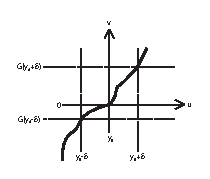
\includegraphics[width=3in]{existence1.eps}
\end{center}

And here is a graph of $u=G^{-1}(v)$:

\begin{center}
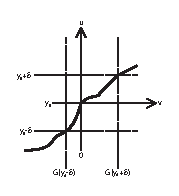
\includegraphics[width=3in]{existence2.eps}
\end{center}


%% Cut below here for the book form.

\begin{center} {\LARGE Problems} \end{center}

\setcounter{problem}{1}

\problem Verify that the functions
\[ y = \left\{ \begin{matrix} 0 & \mbox{for } x \leq a \\ \frac{1}{4}(x-a)^2 & \mbox{for } x > a \end{matrix} \right. \]
for $a>0$ all satisfy the IVP
\[ y'=\sqrt{y}, \ \ \ y(0)=0.\]
Therefore there are infinitely many solutions of the IVP.  Which hypothesis of Theorem 1 is not met in order that this might happen?  {\it (Hint: When you calculate the derivtive of $y$ to check the differential equation, make sure you use the limit definition of derivative at $x=a$.)}






\end{document}